\documentclass[sigconf]{acmart}
\settopmatter{printacmref=false} % Disables ACM reference format
\renewcommand\footnotetextcopyrightpermission[1]{} % Removes the copyright block
\settopmatter{printacmref=false, printccs=false, printfolios=false} % Suppress ACM references
\renewcommand\footnotetextcopyrightpermission[1]{} % Remove copyright
\pagestyle{plain} % Plain header and footer

% added
\usepackage{amsmath}
\usepackage{geometry}
\usepackage{array}
\usepackage{graphicx}  % For resizing the table

% Remove conference information
\acmConference{}{}{} % Clears conference name, location, and date
\acmYear{} % Clears year
\acmISBN{} % Clears ISBN
\acmDOI{} % Clears DOI

\begin{document}

\title{Equivariant Diffusion for Molecule Generation in 3D}

\author{Gaëtan Ecrepont}
\email{gaetan.ecrepont@polytechnique.edu}
\affiliation{%
  \institution{Ecole Polytechnique}
  \city{Paris}
  \country{France}
}

\author{Samson Gourevitch}
\email{samson.gourevitch@polytechnique.edu}
\affiliation{%
  \institution{Ecole Polytechnique}
  \city{Paris}
  \country{France}
}

\author{Samuel Safarti}
\email{samuel.safarti@esade.edu}
\affiliation{%
  \institution{ESADE}
  \city{Paris}
  \country{France}
}

\begin{abstract}
  mettre notre abstract ici
\end{abstract}


\keywords{molecule generation, equivariant network, diffusion models, graph neural networks}


\begin{teaserfigure}
  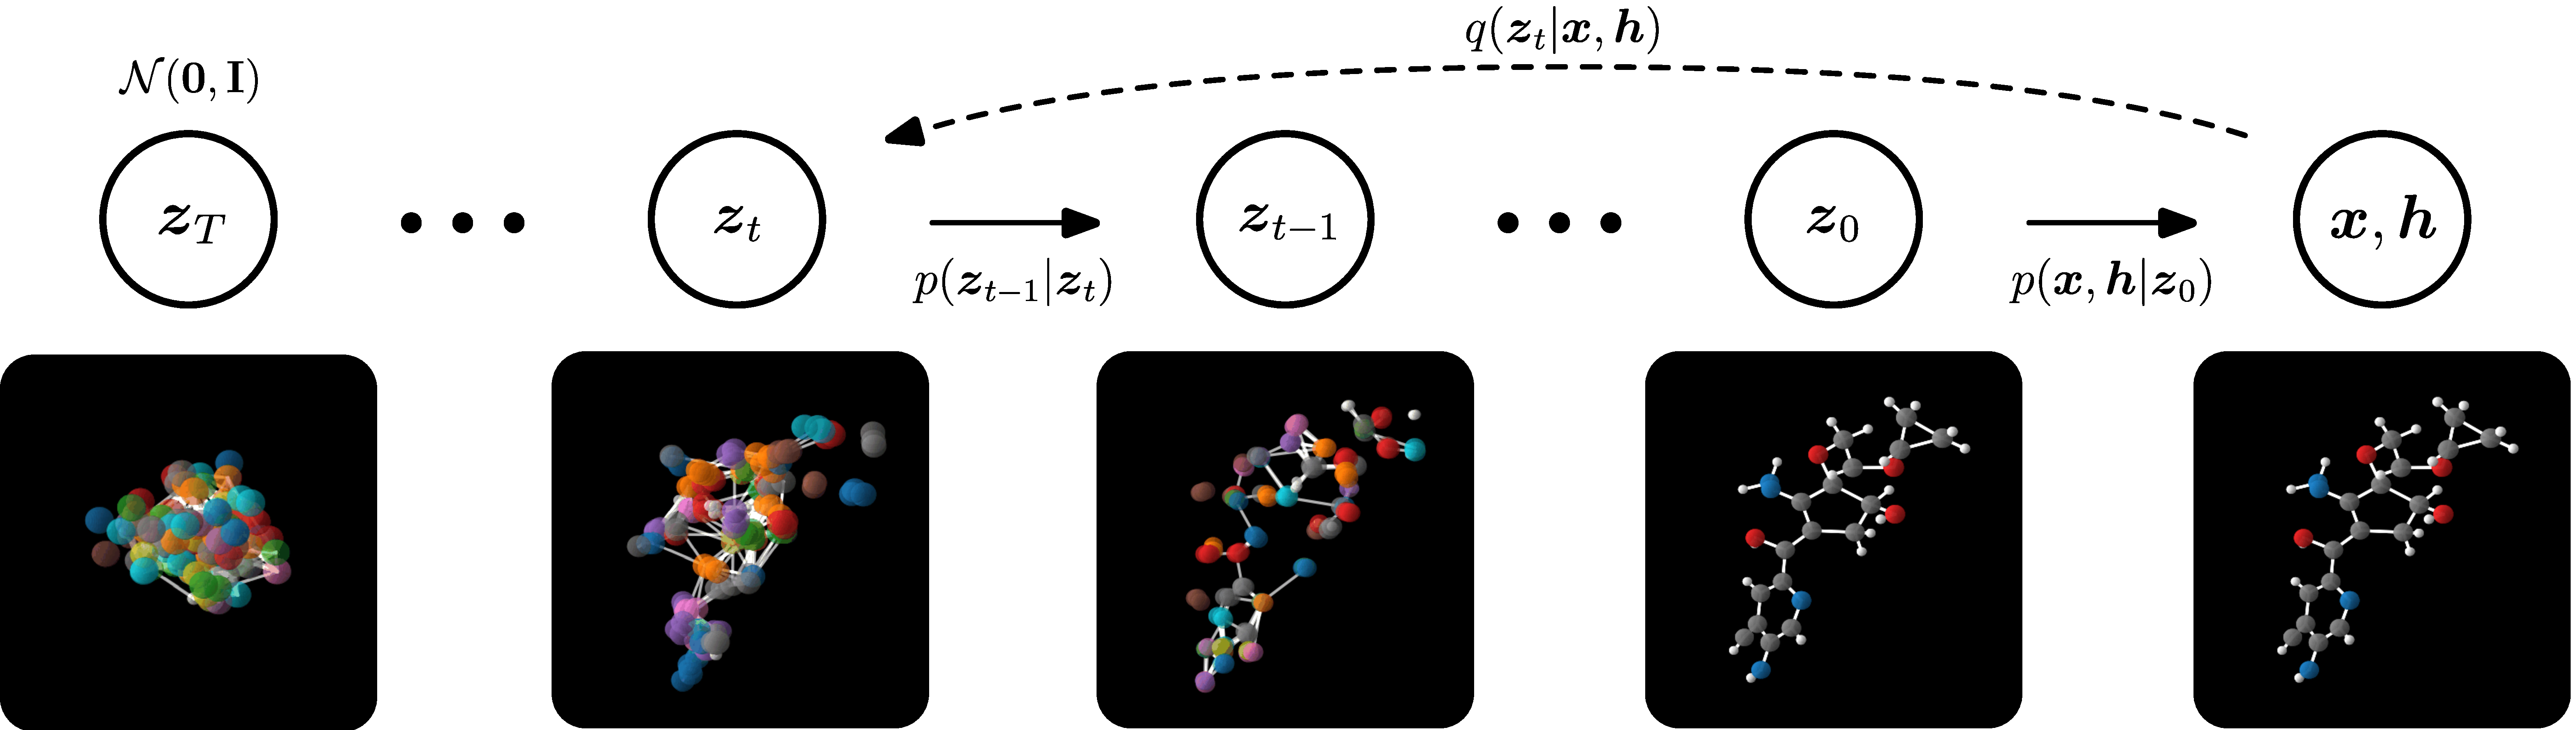
\includegraphics[width=\textwidth]{figures/overview_diffusion.pdf}
  \caption{Overview of the Equivariant Diffusion Model}
  \Description{Overview of the Equivariant Diffusion Model}
  \label{fig:teaser}
\end{teaserfigure}

\received{4 December 2024}

\maketitle

\section{Introduction} %% 1) Context
\subsection{Molecule Generation in 3D}
enjeux globaux; ce qu'on sait faire / ne sait pas faire
\subsection{Existing approaches}
méthodes déjà existantes (e.g. Normalizing Flows, Autoregressive models, etc.): les présenter brièvement et les comparer
\subsection{Proposed approach}
expliquer brièvement (sans rentrer dans les détails) la méthode proposée et ses avantages/inconvénients par rapport aux autres approches


\section{EDM: E(3) Equivariant Diffusion Model} %% 2) Main content
\subsection{Diffusion}
Diffusion models are a class of generative models that operate by iteratively denoising a noised signal.
In essence, diffusion models define a (forward) noising process which diffuses the complex target distribution $p_\text{data}(\mathbf{x})$ into a simple distribution we know how to sample, usually a Gaussian distribution.
The training consists in learning the reverse process, usually by leveraging neural networks which given the noisy signal at step $t$ predict the noise increment so that we can recover the original signal at step $t-1$.
Once the reverse process is learned, one can sample from the target distribution by starting from the simple distribution $\mathbf{x}_T \sim \mathcal{N}(0, I)$ and iteratively denoising it $T$ times to get a sample from the target distribution $\mathbf{x}_0 \sim p_\text{data}(\mathbf{x})$.

Diffusion models were first introduced in the context of image generation by \cite{ddpm} but they can also be applied to generate other modalities such as molecules.
One simple approach to do so is to represent the molecule as a vector $\left[ \mathbf{x}, \mathbf{h} \right]$ where $\mathbf{x} \in (\mathbb{R}^3)^M$ is the position of the atoms in 3D space and $\mathbf{h} \in (\mathbb{R}^\text{nf})^M$ is the atom features.
Here $M$ is the number of atoms in the molecule and $\text{nf}$ is the number of features used to embed the atoms.
In the paper, the atom features are the atom type (H, C, O, N, F one-hot encoded in a 5-dimensional vector) and charge (integer) such that $\text{nf} = 6$.

It makes sense to treat differently the atom positions $\mathbf{x}$ and the atom features $\mathbf{h}$ since the former live in $\mathbb{R}^3$ and are subject to the symmetries of the Euclidean group $E(3)$ while the latter live in $\mathbb{R}^\text{nf}$ and are not subject to these symmetries.
For this reason, the latent space distingues between the atom positions and the atom features by representing the molecule as a vector concatenation $\left[ \mathbf{z}^{(x)}_t, \mathbf{z}^{(h)}_t \right]$.
However, the two vectors do interact in the reverse diffusion process i.e. there is only one diffusion process for the whole molecule.

\begin{figure}
    \centering
    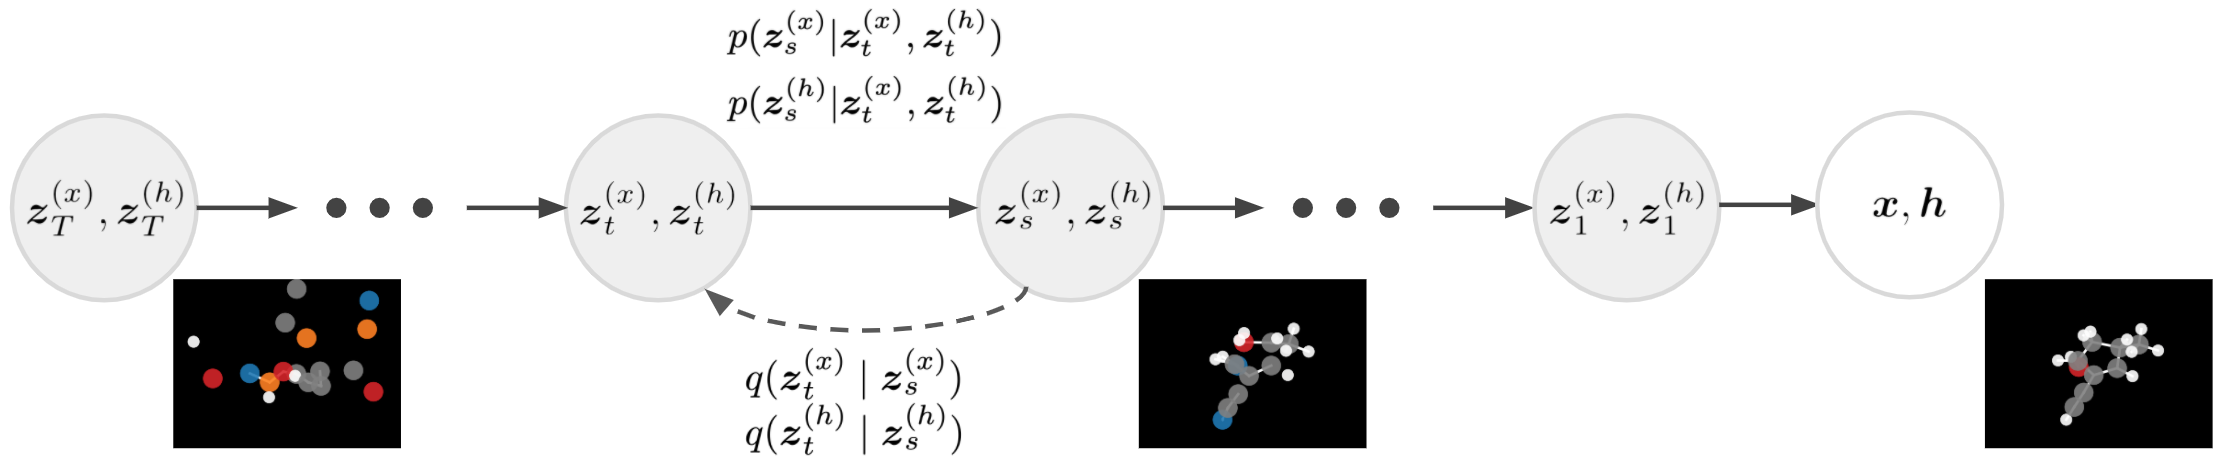
\includegraphics[width=0.25\textwidth]{figures/diffusion.png}
    \caption{The diffusion process of the molecule $\left[ \mathbf{x}, \mathbf{h} \right]$ in the latent space $\left[ \mathbf{z}^{(x)}, \mathbf{z}^{(h)} \right]$.}
    \label{fig:diffusion}
\end{figure}

\subsection{Graph Neural Networks}
Graph Neural Networks (GNNs) are a class of neural networks that operate on graph-structured data.
They are designed to capture the structure of the graph and the interactions between its nodes.
More precisely, a GNN is an optimizable transformation on all attributes of the graph (nodes, edges, and global attributes) 
that preserves graph symmetries. (permutation invariance) \cite{gentle-intro-GNN}

\begin{figure}
    \centering
    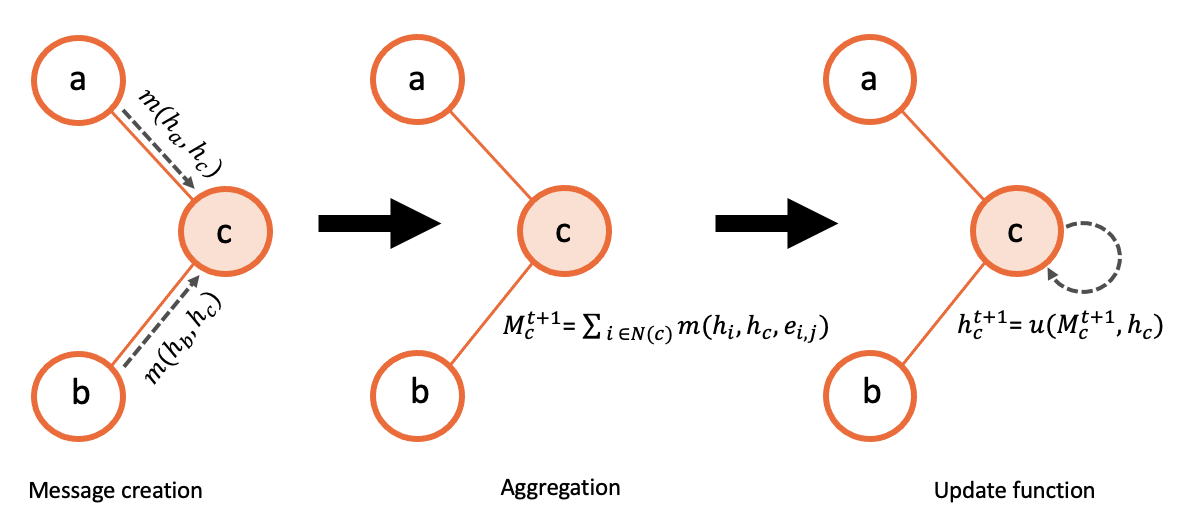
\includegraphics[width=0.25\textwidth]{figures/message_passing.png}
    \caption{The message passing scheme of a GNN.}
    \label{fig:message-passing}
\end{figure}

\subsection{Equivariance, Invariance, and the E(3) group}
Equivariance is a form of symmetry for functions. Roughly speaking, a function is equivariant to a group of transformations $G$ 
if and only if $\forall T\in G, f(T(x)) = T(f(x))$.
Likewise, invariance is when the function is constant under the action of the group i.e. $\forall T\in G, f(T(x)) = f(x)$.
In the context of molecule generation, we are interested in the spatial symmetries of the molecules. Indeed, only the relative positions of the atoms matter, not their absolute positions.
Therefore, we would want our generative model's final output to be invariant to the Euclidean group $E(3)$, which is the group of translations, rotations and reflections in 3D space.
Likewise, since we use diffusion to gradually denoise the molecule, we would want the denoising process to be equivariant to $E(3)$.
This inductive bias is expected to help the model learn the spatial structure of the molecules more efficiently i.e. the model will be able to generalize better and with less training data.

\subsection{E(3) Equivariant GNN}
In their paper, \cite{edm} propose a GNN architecture that is equivariant to the Euclidean group $E(3)$. To do so, they first define an Equivariant 
Graph Convolutional Layer (EGCL) that is equivariant to the Euclidean group $E(3)$. This layer is then stacked to form the Equivariant Graph Neural Network (EGNN).

The EGCL computes $\mathbf{x}^{t+1}, \mathbf{h}^{t+1} = \text{EGCL}(\mathbf{x}^t, \mathbf{h}^t)$ as follows:
\begin{gather}
    \mathbf{m}_{ij} = \phi_e(\mathbf(h)_i^t, \mathbf{h}_j^t, d_{ij}^2), \quad \tilde{e}_{ij} = \phi_{inf}(\mathbf{m}_{ij}) \\
    \mathbf{h}_i^{t+1} = \phi_h(\mathbf{h}_i^t, \sum_{j\neq i} \tilde{e}_{ij} \mathbf{m}_{ij}) \\
    x_i^{t+1} = x_i^t + \sum_{j\neq i} \frac{x_i^t - x_j^t}{d_{ij}+1} \phi_x(\mathbf{h}_i^t, \mathbf{h}_j^t, d_{ij}^2, a_{ij})
\end{gather}
where $\phi_e, \phi_{inf}, \phi_h, \phi_x$ are neural networks and $d_{ij}$ is the Euclidean distance between atoms $i$ and $j$.
Note that $\tilde{e}_{ij}$ implements an attention mechanism for the aggregation of the messages $\mathbf{m}_{ij}$.
Importantly, the EGCL is equivariant to actions the Euclidean group $E(3)$ on the atom positions $\mathbf{x}$ since replacing $\mathbf{x}_i^t$ by $R\mathbf{x}_i^t + t$ for any $R\in SO(3)$ and $t\in \mathbb{R}^3$ results in the same transformation on $\mathbf{x}_i^{t+1}$.
Besides, on can easily show by induction that the EGNN is also equivariant to $E(3)$ since it is a stack of EGCLs.

\subsection{Wrapping it together}
Finally, the Equivariant Diffusion Model (EDM) is obtained by combining the diffusion model and the EGNN.
The training objective is $\mathbb{E}_{t, \epsilon_t}[||\epsilon_t - \hat{\epsilon}_t||^2]$ where $\hat{\epsilon}_t$ i.e. we want to predict the noise.
We use the EGNN to predict the noise increment $\hat{\epsilon}_t$ given the noisy molecule $\left[ \mathbf{x}_t, \mathbf{h}_t \right]$ nad the time step $t$.
To be precise, we set $\hat{\epsilon}_t = \left[ \hat{\epsilon}_t^{(x)}, \hat{\epsilon}_t^{(h)} \right] 
= \text{EGNN}(\mathbf{z}_t^{(x)}, \mathbf{z}_t^{(h)}) - \left[ \mathbf{z}_t^{(x)}, \mathbf{0} \right]$. This recentering trick is necessary for translational equivariance of the EGNN. More details can be found in the original paper \cite{edm}.
Once the EGNN is trained, we can sample from the target distribution by starting from the simple distribution $\mathbf{z}_T \sim \mathcal{N}(0, I)$ and iteratively denoising it $T$ times to get $\mathbf{z}_0$.
We must then decode $\mathbf{z}_0 = \left[ \mathbf{z}_0^{(x)}, \mathbf{z}_0^{(h)} \right]$ to get the molecule $\left[ \mathbf{x}_0, \mathbf{h}_0 \right]$. Doing so is non-trivial since we have continuous (positions), categorical (atom type) and ordinal (charge) variables.
In the paper, the authors use Bayes rule and some approximations to decode $\mathbf{z}_0$.
\begin{itemize}
    \item The atom positions $\mathbf{x}_0$ are obtained by sampling from a gaussian distribution centered around $\mathbf{z}_0^{(x)}$ (plus a correction term)
    \item The atom type is obtained by sampling from a categorical distribution which essentially amounts to taking the nearest one-hot encoded vector to $(\mathbf{z}_0^{(h)})_{1:5}$
    \item The charge is obtained by sampling from a gaussian distribution centered around $(\mathbf{z}_0^{(h)})_6$ which essentially amounts to taking the nearest integer to $(\mathbf{z}_0^{(h)})_6$
\end{itemize}
In addition, the authors use a heuristic distance-based method to create the edges of the molecule. That is, for each pair of atoms $i$ and $j$, they compute the distance $d_{ij}$ 
and based on that distance and a table of bond lengths for these atoms they decide whether there is a bond between $i$ and $j$ and if so what type of bond it is.

Finally, note that since the initial distribution $\mathbf{z}_T \sim \mathcal{N}(0, I)$ is E(3)-invariant
\footnote{Note that no nonzero distribution can be translation invariant, since it wouldn't integrate to one. 
However, one can use distributions on the linear subspace of $(\mathbb{R}^3)^M$ such that the sum $\sum_i \mathbf{x}_i = \mathbf{0}$ i.e. the center of mass of the molecule is at the origin.
Xu et al \cite{xu} showed that such a linear subspace can be used consistently for diffusion.}
and the EGNN is E(3)-equivariant, the final distribution of the model is also E(3)-invariant. (this can be shown easily by induction)

\section{Limitations and extensions} %% 3) Limites et extensions
\subsection{Evaluation Metrics}
critiquer novelty on QM9 / molecule stability on GEOM / NLL on both / Wasserstein distance on histograms
\subsection{E(3) vs. SE(3) equivariance}
expliquer pourqoi SE(3) pourrait être mieux/moins bien + voir ce qui a été fait dans la littérature
\subsection{Adding the edges to the models}
justifier la pertinence/les difficultés d'une intégration des edge types (none, simple, double, triple bond) dans la diffusion latente --> c'est a priori mieux que l'heuristique distance-based pour créer des liaisons à la fin? Voir littérature!
\subsection{Choice of M}
Critiquer le fait qu'il faille fixer M pour générer! Peut-on faire autrement? (maybe not?)

\section{Experiments on toy model}
The key contribution of the Hoogeboom's paper is the introduction of E(3)-equivariance in Graph Neural Networks.
Reproducing the paper's experiment is not computationally feasible for students as training takes about 7 days on GPUs. However, we can study the advantage of E(3)-equivariant GNNs over regular GNNs with simpler experiments. We shift our focus from a generation to a regression class, which is less resource intensive and sufficient to demonstrate the superior performance of equivariant models over vanilla ones.
We first present the dataset used and then the models considered. We then disxplay our results and discuss them.

\subsection{Dataset}
The paper considers two molecule datasets: QM9 and GEOM. We will stick with QM9 at it is simpler (smaller molecules). Since QM9 has over 100,000 molecules, we filter to keep only molecules with 12 atoms or less. This brings us down to 4005 molecules.
Each sample in the dataset is a graph with several properties:
\begin{itemize}
    \item number of atoms $M$
    \item atom positions $\mathbf{x} \in (\mathbb{R}^3)^M$
    \item atom features $\mathbf{h} \in (\mathbb{R}^\text{nf})^M$ where $\text{nf} = 11$
    \begin{itemize}
        \item 1-5: atom type (one-hot: H, C, O, N, F)
        \item 6: atomic number (number of protons)
        \item 7: aromaticity (binary)
        \item 8-10: electron orbital hybridization (one-hot: sp, sp2, sp3)
        \item 11: number of hydrogens
    \end{itemize}
    \item graph edges (bonds) $\mathcal{E} \in \mathbb{R}^{2\times\text{\#edges}}$
    \item edge features $\mathcal{E}_\text{type} \in \mathbb{R}^{\text{\#edges}\times 4}$ (one-hot: single, double, triple, aromatic)
\end{itemize}

The QM9 dataset has 19 regression targets which are various physical properties of the molecules.
We will focus on the first target which is the dipole moment of the molecule. We chose this target because it is typically geometric so we expect to clearly see the benefits of 
incorporating E(3)-equivariance in the model.
We adopt a random split of 80\% training, 10\% validation, and 10\% test.
Finally, we normalize our regression target to have zero mean and unit variance.

\subsection{Layers}

All GNNs considered follow the same architecture:
\begin{enumerate}
    \item Linear layer to embed the atom features (which include the atom positions for MPNN): $(M,\text{nf}) \rightarrow (M, d_\text{embed})$
    \item Stacked GCL or EGCL layers (depending on the model) with $L$ layers: $(M, d_\text{embed}) \rightarrow (M, d_\text{embed})$
    \item Global mean pooling to aggregate the node features: $(M, d_\text{embed}) \rightarrow (d_\text{embed})$
    \item Linear layer to predict the regression target $(d_\text{embed},) \rightarrow (1,)$
\end{enumerate}

Let's first describe the two types of layers considered.

The GCL layer computes $\mathbf{h}^{t+1} = \text{GCL}(\mathbf{h}^t)$ as follows:
\begin{enumerate}
    \item message $\mathbf{m}_{ij} = \phi_\mathbf{h}(\mathbf{h}_i, \mathbf{h}_j, \mathcal{E}_{ij})$
    \item aggregation $\mathbf{m}_i = \sum_{j\in\mathcal{N}(i)} \mathbf{m}_{ij}$ where $\mathcal{N}(i)$ is the set of neighbors of node $i$
    \item update $\mathbf{h}_i^{t+1} = \phi_\text{update}(\mathbf{h}^t, \mathbf{m}_i)$
\end{enumerate}

The EGCL layer computes $\mathbf{h}^{t+1}, \mathbf{x}^{t+1} = \text{EGCL}(\mathbf{h}^t, \mathbf{x}^t)$ as follows:
\begin{enumerate}
    \item message
    \begin{align*}
      \mathbf{m}_{ij}^\mathbf{h} &= \phi_\mathbf{h}(\mathbf{h}_i, \mathbf{h}_j, d_{ij}^2) \\
      \mathbf{m}_{ij}^\mathbf{x}& = \frac{\mathbf{x}_i - \mathbf{x}_j}{d_{ij}+1} \phi_\mathbf{x}(\mathbf{h}_i, \mathbf{h}_j, d_{ij}^2)
    \end{align*}
    \item aggregation
    \begin{align*}
      \mathbf{m}_i^\mathbf{h} &= \sum_{j\in\mathcal{N}(i)} \phi_\text{attention}(\mathbf{m}_{ij}) \mathbf{m}_{ij}^\mathbf{h} \\
      \mathbf{m}_i^\mathbf{x} &= \sum_{j\in\mathcal{N}(i)} \mathbf{m}_{ij}^\mathbf{x}
    \end{align*}
    \item update
    \begin{align*}
      \mathbf{h}_i^{t+1} &= \phi_\text{update}(\mathbf{h}_i^t, \mathbf{m}_i^\mathbf{h}) \\
      \mathbf{x}_i^{t+1} &= \mathbf{x}_i^t + \mathbf{m}_i^\mathbf{x}
    \end{align*}
\end{enumerate}

All the functions $\phi_\bullet$ are fully connected neural networks following the same architecture as in the original paper.
Both layers are trivially permutation equivariant. Besides, one can easily show that the EGCL is E(3)-equivariant 
i.e. $\mathbf{h}^t, R\mathbf{x}^t + \mathbf{t} = \text{EGCL}(\mathbf{h}^t, R\mathbf{x}^t + \mathbf{t})$ 
for all orthogonal matrix $R\in O(3)$ and translation vector $\mathbf{t} \in \mathbb{R}^3$.

Since our GNNs have stacked permutation-equivariant layers and then a permutation-invariant global mean pooling, they are permutation-invariant.
Likewise, since the EGCL is E(3)-equivariant and the global mean pooling is permutation-invariant, the E3EGNN is E(3)-invariant.


\subsection{Models}

Taking inspiration from \cite{gnn-101}, we consider the following models:
\begin{itemize}
    \item MPNN: a Message Passing Neural Network (MPNN) built with stacked Graph Convolutional Layers (GCL)
    \item EGNN: an E(3)-equivariant GNN built with stacked E(3)-Equivariant Graph Convolutional Layers (EGCL)
    \item EGNN\_edge: same architecture as EGNN but using the edge features $\mathcal{E}_\text{type}$ as well when computing the messages
\end{itemize}
All models have $L=4$ layers and $d_\text{embed}=11$ (i.e. the same as the input dimension).
We also consider LinReg, a linear regression model (projects each atom to a scalar and sums them up to get the final prediction), for baseline comparison with the geometric models.
We expect poor performance as it doesn't leverage the graph structure of the molecules.

\begin{table}[h!]
\centering
\resizebox{0.5\textwidth}{!}{ % Resize the table to fit the text width
\begin{tabular}{|l|l|l|l|l|} \hline
\textbf{Model} & \textbf{Perm-Eq Layers} & \textbf{Perm-Inv} & \textbf{E(3)-Eq Layer} & \textbf{E(3)-Inv} \\ \hline
MPNN            & Yes                     & No                 & No                     & Yes                \\ \hline
EGNN            & Yes                     & Yes                & Yes                     & Yes                \\ \hline
EGNN\_edge      & Yes                     & Yes                & Yes                     & Yes                \\ \hline
LinReg          & Yes                     & No                 & No                     & Yes                \\ \hline
\end{tabular}
}
\caption{Symmetry Properties of the Different Models}
\end{table}

\subsection{Implementation details}
\begin{itemize}
    \item We use PyTorch Geometric to handle the graph data
    \item We use the Adam optimizer with a learning rate of $10^{-3}$ and a batch size of 64
    \item We use the ReduceLROnPlateau scheduler with a patience of 10 epochs, a factor of 0.9, and a minimum learning rate of $10^{-5}$
    \item We train each model for 500 epochs
    \item We use the mean squared error as the loss function
    \item We keep track of the learning rate, training loss and validation loss using WandB
    \item We train locally on CPU for simplicity. Each run is about 20 minutes on i7 with 8 cores.
\end{itemize}

\begin{figure}
    \centering
    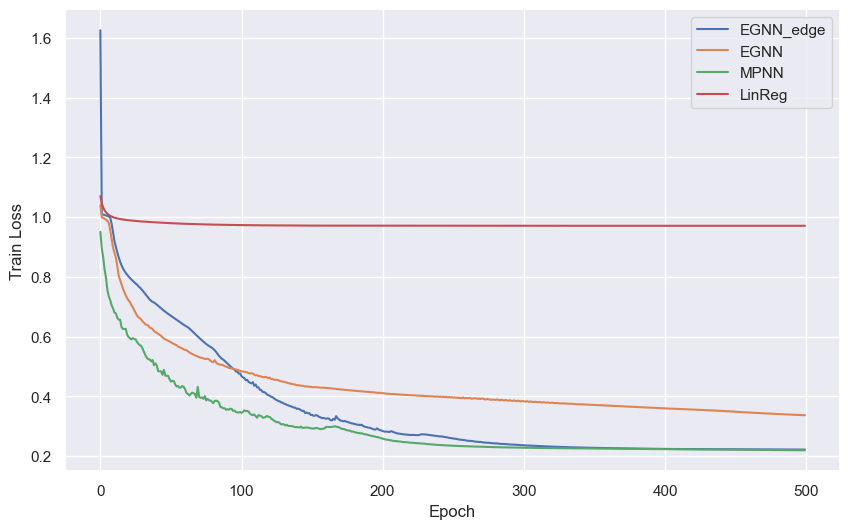
\includegraphics[width=0.42\textwidth]{figures/train_loss.png}
    \caption{Training loss. The LinReg model cannot even overfit the training data, illustrating the superiority of a graph-based approach.}
    \label{fig:training-loss}
\end{figure}

\begin{figure}
    \centering
    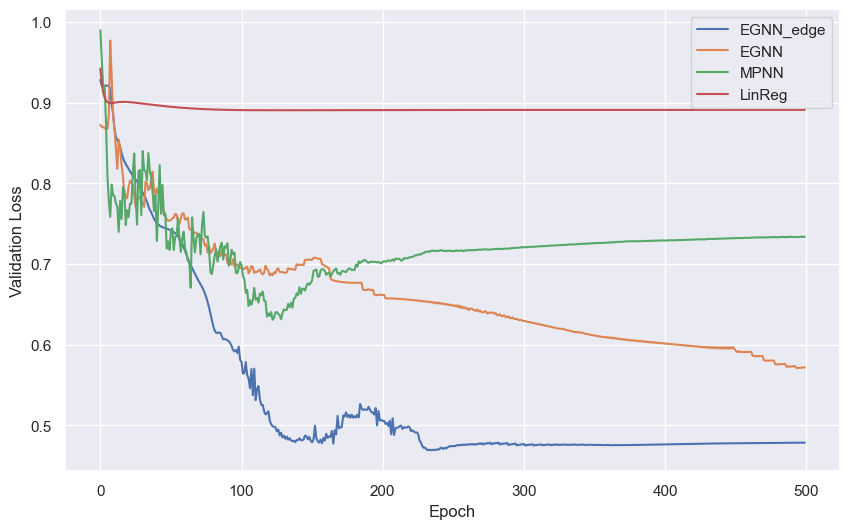
\includegraphics[width=0.42\textwidth]{figures/validation_loss.png}
    \caption{Validation loss. As expected, the EGNN models significantly outperform the MPNN model. In addition, the EGNN model lags behind the EGNN\_edge model, suggesting that incorporating edge features is beneficial.}
    \label{fig:validation-loss}
\end{figure}

\begin{figure}
    \centering
    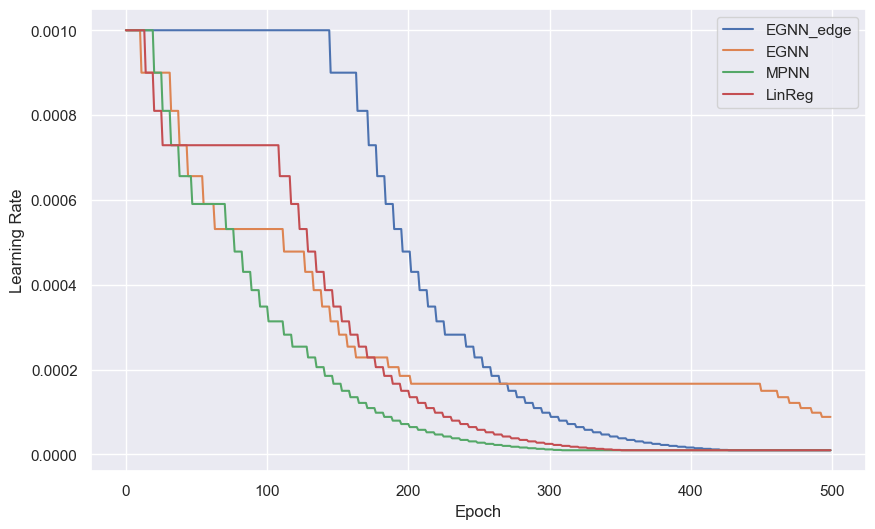
\includegraphics[width=0.42\textwidth]{figures/learning_rate.png}
    \caption{Learning Rate. All models have converged to a local minimum after 500 epochs, except the EGNN which is almost there.}
    \label{fig:learning-rate}
\end{figure}

\subsection{Comments}
The results are reported on three figures: the training loss, the validation loss, and the learning rate.

To begin with, the LinReg model performs very poorly as expected. Unlike its geometric counterparts, it cannot leverage the graph structure of the molecules and thus fails to learn anything meaningful.

Then, MPNN and EGNN\_edge have similar training losses but EGNN\_edge drastically outperforms MPNN on the validation set. This gap shows that EGNN\_edge's inductive bias helps it generalize better than MPNN.

Finally, EGNN is also significantly better than MPNN but learn much slower than EGNN\_edge. This suggests that incorporating edge features is beneficial for the model's performance.
Nonetheless, edge features can intuitively be inferred from the atom positions and types (using a distance-based heuristic like in the original paper), so the improvement is not as significant as the one brought by E(3)-equivariance.
That would explain why the EGNN is still learning and could potentially be as good as EGNN\_edge with more training. To verify this hypothesis, we trained the model for 1000 epochs, but the validation loss and training loss actually plateau around 500 epochs.
Perhaps with more layers or a higher embedding dimension, the EGNN could iner the edge types and thus catch up with EGNN\_edge.


\bibliographystyle{ACM-Reference-Format}
\bibliography{biblio}

\end{document}
